% !TEX program = pdflatex
% Method-and-experiment core draft in the standard IEEE Transactions journal format.
\documentclass[journal]{IEEEtran}

\usepackage{amsmath,amssymb,amsfonts}
\usepackage{bm}
\usepackage{mathtools}
\usepackage{graphicx}
\usepackage{booktabs}
\usepackage{array}
\usepackage{placeins}
\usepackage{xcolor}
\usepackage{cite}
\usepackage[nameinlink,capitalize]{cleveref}

\newcommand{\SMPCC}{S-MPCC}
\newcommand{\MPCC}{MPCC}
\newcommand{\xr}{\bm{x}_{r}}
\newcommand{\xl}{\bm{x}_{\ell}}
\newcommand{\xaug}{\bm{x}}
\newcommand{\vu}{\bm{u}}
\newcommand{\vr}{\bm{r}}
\newcommand{\ec}{e_{\mathrm{c}}}
\newcommand{\el}{e_{\mathrm{l}}}
\newcommand{\Pending}{\textcolor{spmpcgray}{\textit{pending}}}

\definecolor{spmpcgray}{RGB}{90,90,90}

\title{\SMPCC: Slosh-Aware Online Trajectory Generation for Prescribed-Path Liquid Transport}

\author{Renjun Zhang%
\thanks{Renjun Zhang is with the University of Science and Technology of China,
Hefei, China (e-mail: zhangrenjun@mail.ustc.edu.cn).}}

\begin{document}

\maketitle

\begin{abstract}
Transporting an open liquid on a mobile base requires more than suppressing command variation: the response to a candidate motion also depends on the liquid displacement, velocity, and oscillation phase already present when that motion is planned.
This paper presents \SMPCC{}, a receding-horizon trajectory generator and controller for prescribed geometrically feasible paths.
It augments an acceleration-level \MPCC{} with finite-horizon virtual path progress and a container-parameterized first lateral sloshing mode represented in two orthogonal directions.
An odometry-driven model propagates an internal modal state between control cycles, and this model state conditions the next virtual-progress and chassis action; it is not a measurement of the true signed liquid phase.
The evaluation is designed to contrast \SMPCC{} with slosh-agnostic, smooth-only, completion-time-matched, and model-informed fixed-profile conditions using calibrated vision, odometry-derived executed timing, constructed internal modal-phase studies, online-input/zero-state replay, and execution-chain and runtime audits.
Formal outcome claims and numerical results are intentionally withheld until the preregistered release, measurement, comparator, and analysis gates have passed.
The scope is online trajectory generation along a supplied path; global route planning, obstacle reasoning, and a formal spill-free guarantee are not claimed.
\end{abstract}

\begin{IEEEkeywords}
mobile robots, open-liquid transport, liquid sloshing, model predictive contouring control, prescribed-path trajectory generation, online virtual path-progress optimization
\end{IEEEkeywords}

\section{Phase-Rejoining Residual \SMPCC{} Method}
\label{sec:method}

\subsection{Problem, Core Idea, and Scope}

We consider a differential-drive mobile base carrying an open liquid along a geometrically feasible path that is fixed before motion.
An offline anti-slosh sequence can coordinate an initial excitation with a later cancellation, slowdown, and settling tail.
A conventional online tracker may nevertheless alter the speed or turn rate to reduce an immediate path error and thereby invalidate the remaining cancellation.
The central design rule is therefore:
\emph{an online residual may correct tracking, but it is admitted only if the state predicted after the real execution delays remains eligible to rejoin the phase-indexed offline tail.}

Figure~\ref{fig:core_architecture} shows the resulting offline--online structure.
The offline layer owns the complete nominal motion and tail.
The online layer aligns the available state to the expected publication epoch, selects one nearby monotone artifact phase, and optimizes a bounded residual through the unequal linear and angular execution delays.
At the terminal prediction step, a 9-D robot--liquid empirical gate and a compatibility set for the pending execution state must both hold.
This is a hard admission test, not an additional soft slosh penalty.

\begin{figure*}[t]
  \centering
  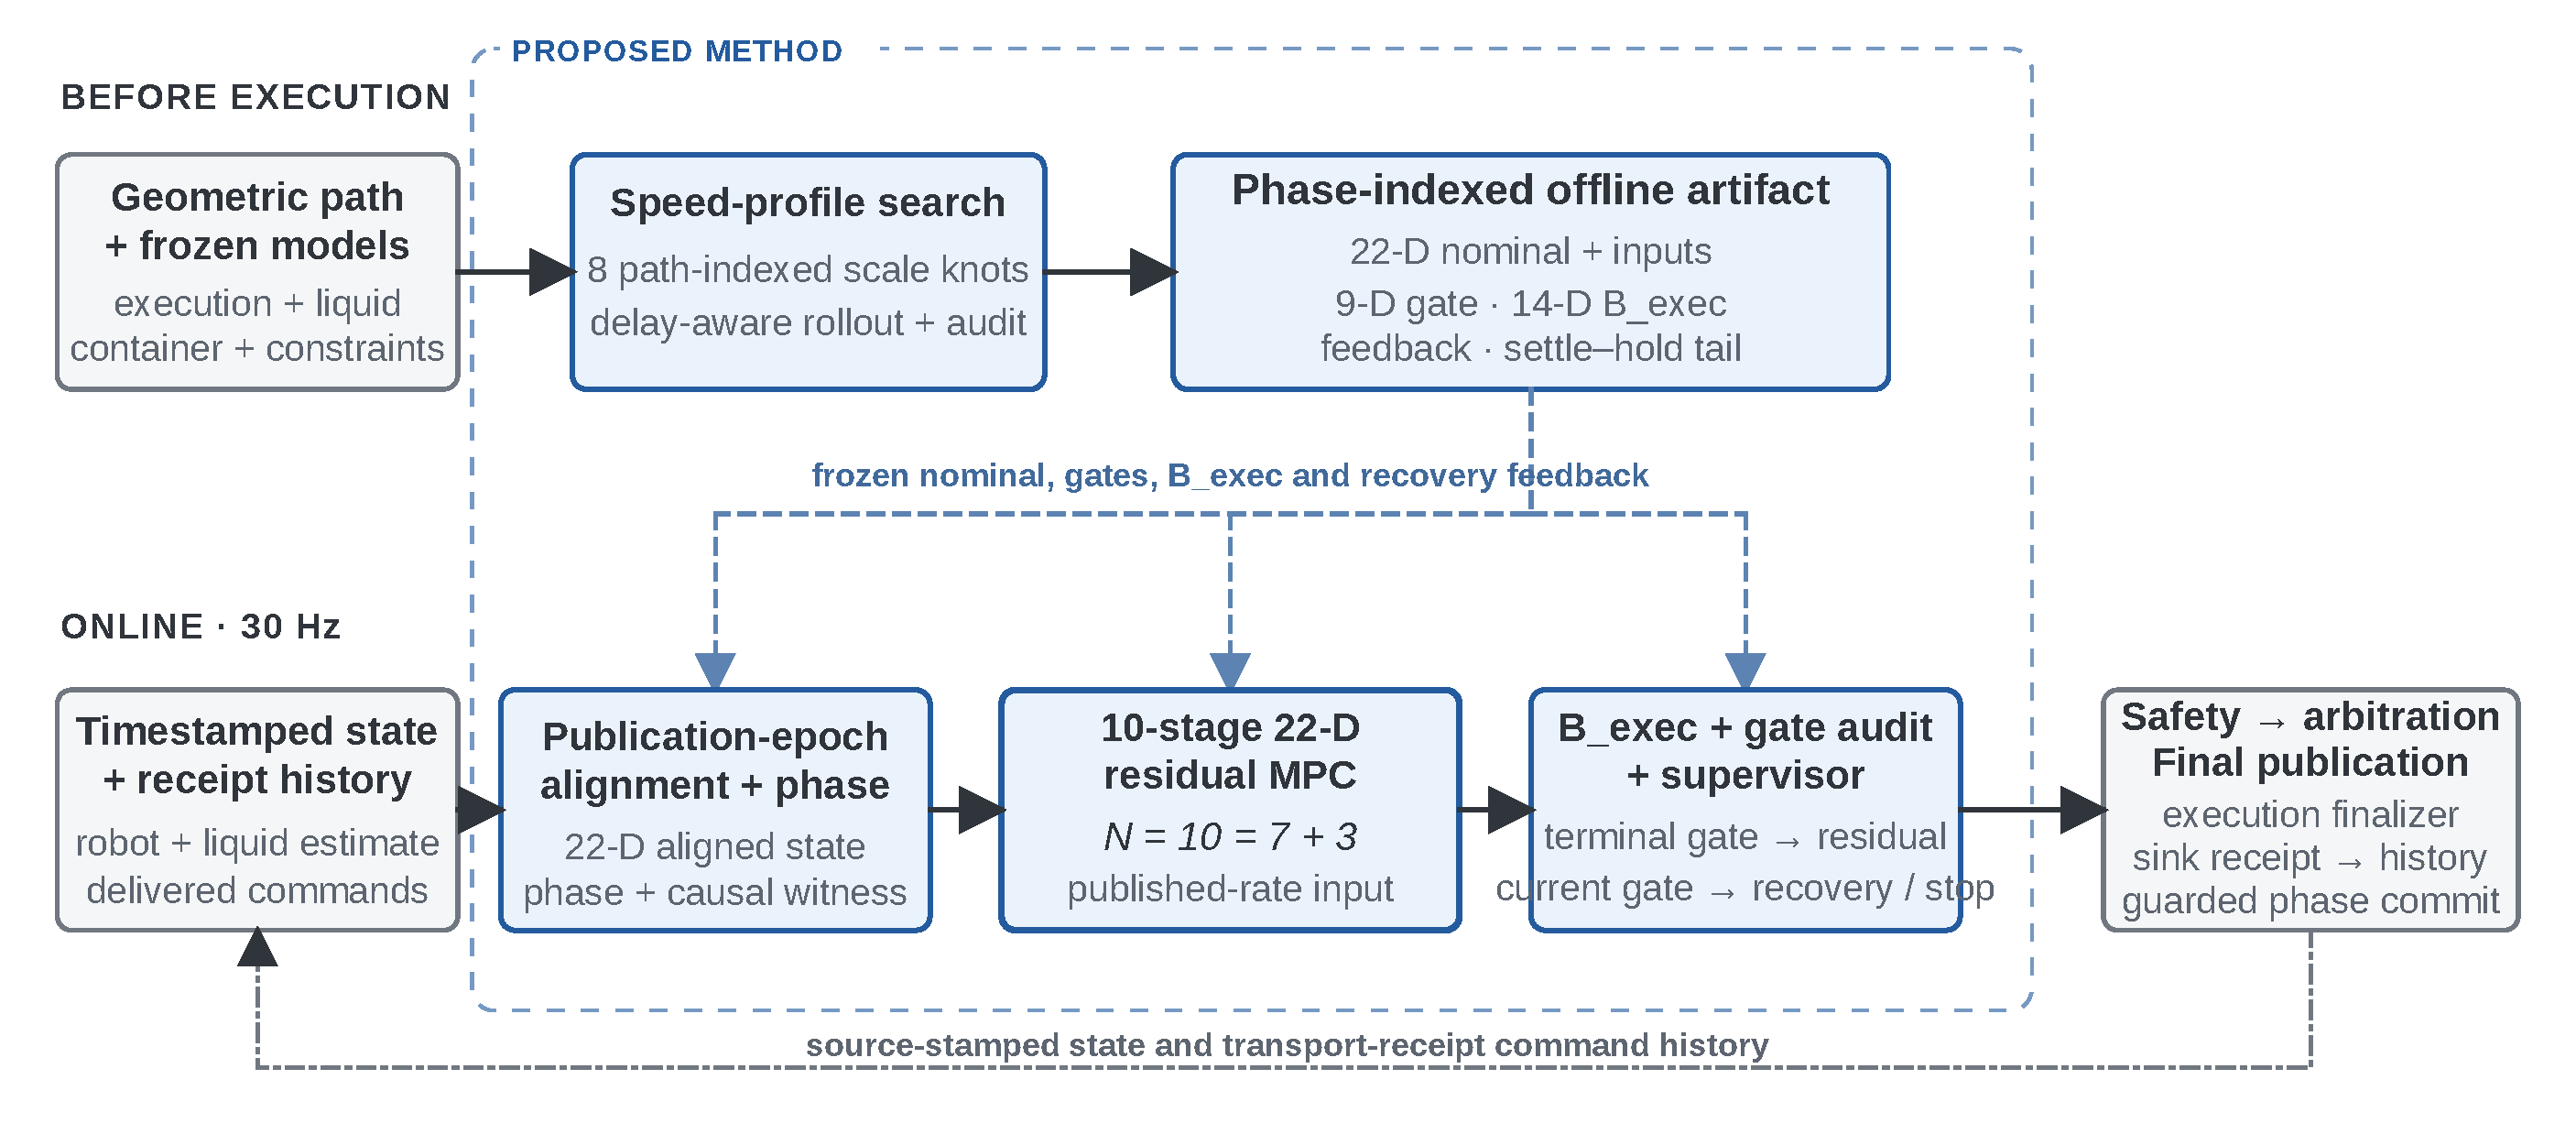
\includegraphics[width=\textwidth]{figures/phase_rejoining_framework_paper.pdf}
  \caption{Overview of \PRSMPCC{}.
  Before execution, OfflineSloshOCP turns the fixed path and frozen execution--liquid models into a phase-indexed artifact with a complete motion--settle--hold tail.
  Online, the state estimate is aligned with the execution front and a nearby monotone phase, and only bounded residuals that pass the joint rejoin test are admitted.
  The supervisor selects residual, recovery, or stop before the common safety and publication chain; measured response and the final published-command history close the loop.}
  \label{fig:core_architecture}
\end{figure*}

The scope is deliberately narrow: a frozen path, a frozen container/model contract, an initially admitted liquid state, and small runtime deviations.
The method performs no online obstacle detection, collision-corridor optimization, homotopy search, or replanning.
An MBF path may be generated before a trial, but its point sequence, frame, and hash must then be frozen and a path-specific offline artifact regenerated.

\subsection{Shared Model and Offline Artifact}

\subsubsection{Robot--liquid and execution state}

Let $\bm p=[p_x,p_y]^\top$ and $\psi$ denote planar position and yaw, and let $v^r$ and $\omega^r$ denote realized linear and angular motion.
For a reference curve $\bm r(s)$ with tangent angle $\psi_r(s)$, the usual lag and contour errors are
\begin{equation}
  \begin{bmatrix}e_l\\e_c\end{bmatrix}
  =
  \begin{bmatrix}
    \cos\psi_r & \sin\psi_r\\
    -\sin\psi_r & \cos\psi_r
  \end{bmatrix}
  \left(\bm p-\bm r(s)\right).
  \label{eq:contour_lag_errors}
\end{equation}
The progress variable $s$ is retained only locally around the selected offline phase; it is not a free global time-scaling variable as in a conventional unconstrained virtual-progress formulation \cite{D19_Liniger2015,D20_Brito2019}.

The liquid model retains the first lateral mode in two orthogonal container axes,
\begin{equation}
  z^\ell=
  [\eta_x,\dot\eta_x,\eta_y,\dot\eta_y]^\top,
  \qquad
  \dot z^\ell=A_\ell z^\ell+B_\ell
  \begin{bmatrix}\dot v^r\\v^r\omega^r\end{bmatrix},
  \label{eq:liquid_model}
\end{equation}
where $A_\ell$ and $B_\ell$ are obtained from the frozen container and liquid parameters.
This low-order representation follows equivalent mechanical slosh models used for two-dimensional excitation \cite{A01_Leva2021,A02_Guagliumi2021}.
It is an internal prediction state, not a direct measurement of the true signed liquid phase.

We distinguish three state descriptions:
\begin{align}
  \chi &=[p_x,p_y,\psi,v^r,\omega^r,z^{\ell\top}]^\top\in\mathbb R^9,
  \label{eq:gate_state}\\
  X &=\operatorname{col}(p_x,p_y,\psi,v^c,s,\omega^c,z^\ell),
  \label{eq:base_ocp_state}\\
  X^{\mathrm{aug}}&=\operatorname{col}(X,b^v,b^\omega,x^a).
  \label{eq:augmented_state}
\end{align}
For phase selection and gate construction, yaw is never subtracted as an unwrapped Euclidean coordinate.
We use the common 9-D error operator
\begin{equation}
\begin{split}
  \mathcal E_\chi(\chi,\bar\chi)=\operatorname{col}\big(&
  \bm p-\bar{\bm p},
  \operatorname{wrap}_{(-\pi,\pi]}(\psi-\bar\psi),\\
  &v^r-\bar v^r,\ \omega^r-\bar\omega^r,\
  z^\ell-\bar z^\ell\big).
\end{split}
\label{eq:gate_error_operator}
\end{equation}
Here $v^c$ and $\omega^c$ are command-integrator states, $b^v$ and $b^\omega$ are the linear and angular command buffers, and $x^a=[v^r,\omega^r]^\top$ contains the realized actuator states.
The acceleration-level OCP input is
\begin{equation}
  q=[a,\alpha,v_s]^\top,
  \label{eq:ocp_input}
\end{equation}
with linear acceleration $a$, angular acceleration $\alpha$, and local progress rate $v_s$.
Within the horizon, $q_k$ first generates a raw solver command and its hypothetical publishable counterpart,
\begin{align}
  u_k^{\mathrm{sol}}
  &=\begin{bmatrix}v_k^c+a_k\Delta t\\
                     \omega_k^c+\alpha_k\Delta t\end{bmatrix},
  \label{eq:solver_command_map}\\
  u_k^{\mathrm{pred}}
  &=\Pi_{\mathrm{cmd}}(u_k^{\mathrm{sol}},b_k^v,b_k^\omega),
  \label{eq:predicted_publishable_command}
\end{align}
where $\Pi_{\mathrm{cmd}}$ applies the frozen speed, acceleration, and rate limits modeled by the OCP.
It does not predict an independent safety override.
The command and local-progress states then satisfy
\begin{equation}
  \begin{bmatrix}v_{k+1}^c\\\omega_{k+1}^c\end{bmatrix}
  =u_k^{\mathrm{pred}},
  \qquad
  s_{k+1}=s_k+\Delta t\,v_{s,k}.
  \label{eq:command_progress_update}
\end{equation}

For channel $r\in\{v,\omega\}$, write
\begin{equation}
  m_r=\left\lfloor\frac{d_r}{\Delta t}\right\rfloor,
  \qquad
  \lambda_r=\frac{d_r}{\Delta t}-m_r.
  \label{eq:fractional_delay}
\end{equation}
The predicted FIFO shift and fractionally delayed setpoint are
\begin{align}
  b_{k+1}^{r,(0)}&=u_{r,k}^{\mathrm{pred}},
  &b_{k+1}^{r,(h+1)}&=b_k^{r,(h)},
  \label{eq:buffer_shift}\\
  \widetilde u_{r,k+1}
  &=(1-\lambda_r)b_{k+1}^{r,(m_r)}
    +\lambda_r b_{k+1}^{r,(m_r+1)},
  \label{eq:fractional_delay_output}
\end{align}
with $h=0{:}m_r$ and buffer entries $0{:}m_r+1$.
With identified gain $g_r$ and time constant $\tau_r$, the actuator update is
\begin{equation}
  x^a_{r,k+1}=\gamma_r x^a_{r,k}
  +(1-\gamma_r)g_r\widetilde u_{r,k+1},
  \qquad
  \gamma_r=e^{-\Delta t/\tau_r}.
  \label{eq:actuator_update}
\end{equation}
The realized $v^r=x_v^a$ and $\omega^r=x_\omega^a$ drive the base kinematics and the excitation in \eqref{eq:liquid_model}; in discrete time,
\begin{align}
  \bm p_{k+1}&=\bm p_k+\Delta t\,v_k^r
  [\cos\psi_k,\sin\psi_k]^\top,
  &\psi_{k+1}&=\psi_k+\Delta t\,\omega_k^r,
  \label{eq:realized_kinematics}\\
  a_{x,k}^r&=(v_{k+1}^r-v_k^r)/\Delta t,
  &a_{y,k}^r&=v_k^r\omega_k^r.
  \label{eq:realized_excitation}
\end{align}
Equations~\eqref{eq:solver_command_map}--\eqref{eq:realized_excitation}, the local progress update, and the discretized liquid model define
\begin{equation}
  X^{\mathrm{aug}}_{k+1}
  =F_{\mathrm{exec}\text{-}\ell}
  \left(X^{\mathrm{aug}}_k,u_k^{\mathrm{pred}},v_{s,k};\Theta\right),
  \label{eq:delay_augmented_dynamics}
\end{equation}
where $\Theta$ freezes the robot, liquid, unequal delay, buffer, and actuator parameters.

The superscript ``pred'' is confined to a hypothetical OCP rollout.
After supervision and all runtime overrides, the measured $u^{\mathrm{pub}}$ is the only command appended to the persistent buffers and used for delay identification; an unexecuted $u^{\mathrm{sol}}$ or $u^{\mathrm{pred}}$ is never written into command history.
At the next solve, the command-integrator state is reanchored to the latest final $u^{\mathrm{pub}}$ before constructing the rollout.

\subsubsection{Complete \OfflineSloshOCP{} artifact}

Input shaping and offline anti-slosh planning can exploit the complete motion rather than a truncated online preview \cite{A07_Singer1990,B03_Hamaguchi2004,B02_Hamaguchi2005,C01_Ferrari2026}.
For the frozen path and contract, \OfflineSloshOCP{} produces
\begin{equation}
  \bar{\mathcal A}=\left(
  \{\bar X_i^{\mathrm{aug}},\bar\chi_i,\bar t_i\}_{i=0}^{M},
  \{\bar q_i,\bar u_i^{\mathrm{pub}}\}_{i=0}^{M-1}
  \right).
  \label{eq:offline_artifact}
\end{equation}
Unlike a trajectory truncated at geometric arrival, $\bar{\mathcal A}$ includes motion, slowdown, liquid settling, and a verified zero-command hold.
The nominal buffer and actuator states are generated by passing the nominal published commands through the same execution model used online.
At the paper level, the offline problem is
\begin{subequations}
\label{eq:offline_ocp_contract}
\begin{align}
  \min_{\{\bar X_i^{\mathrm{aug}},\bar q_i\}}
  \quad &
  \bar J_{\mathrm{task}}+\bar J_{\mathrm{liquid}}
  +\bar J_{\mathrm{regularity}},
  \label{eq:offline_ocp_objective}\\
  \text{s.t.}\quad &
  \bar X_{i+1}^{\mathrm{aug}}
  =F_{\mathrm{exec}\text{-}\ell}
  (\bar X_i^{\mathrm{aug}},\bar u_i^{\mathrm{pred}},\bar v_{s,i};\Theta),
  \label{eq:offline_ocp_dynamics}\\
  &(\bar X_i^{\mathrm{aug}},\bar q_i)\in\mathcal Z,
  \label{eq:offline_ocp_constraints}\\
  &\bar u_i^{\mathrm{pub}}=(0,0),
  \quad i=M-N_h{:}M-1,
  \label{eq:offline_zero_hold}\\
  &\|\bar z_i^\ell\|\le\epsilon_{\mathrm{settle}},
  \quad i=M-N_h{:}M.
  \label{eq:offline_tail_constraint}
\end{align}
\end{subequations}
The three costs cover prescribed-path completion, modeled liquid response including the tail, and command regularity; their frozen definitions and weights belong to the supplementary release record.
$N_h$ and $\epsilon_{\mathrm{settle}}$ define the terminal zero hold before any formal artifact is built.

Each artifact phase $i$ additionally stores
\begin{equation}
  \left(
  \widehat{\mathcal R}^{\mathrm{emp}}_i,
  \mathcal B_i^{\mathrm{exec}},
  u_{\mathrm{rec}}(i)
  \right),
  \label{eq:phase_objects}
\end{equation}
where $\widehat{\mathcal R}^{\mathrm{emp}}_i$ is a 9-D empirical recovery gate, $\mathcal B_i^{\mathrm{exec}}$ is an execution-state compatibility set, and $u_{\mathrm{rec}}(i)$ is a phase-indexed stored action.
The artifact contract freezes the path and frame hashes, time grid, robot/execution/liquid models, container and fill range, constraints, complete tail, gate schema, and software version.
A change to any contracted object invalidates the artifact rather than silently reusing it.

The empirical objects are constructed from recovery rollouts around each phase.
A sample is labeled successful only when its execution state is compatible, the stored action is applied through the publication chain, the nominal tail is resumed, all constraints remain satisfied, and the preregistered settling rule is met.
On $D_{\mathrm{gate,fit}}$, a finite stored-action library and candidate values of $\rho_{r,i}$ and $\beta^{\mathrm{exec}}_{r,i}$ are evaluated by a frozen selection rule.
The target rule maximizes accepted coverage subject to minimum per-phase support and a preregistered upper confidence bound on the conditional false-safe fraction; a phase with no admissible candidate is marked unavailable.
The selected $u_{\mathrm{rec}}(i)$, radii, bounds, and unavailable phases are frozen before $D_{\mathrm{gate,test}}$ is opened.

\subsection{Execution-Front Alignment and Phase Rejoining}

\subsubsection{Expected publication epoch and unequal delays}

Let $t_s$ be the source timestamp of the latest admitted state and $t_c$ the start of the current computation.
With the frozen or online estimate $\widehat d_c$ of computation-to-publication delay, the prediction epoch is
\begin{equation}
  t=t_c+\widehat d_c,
  \label{eq:publication_epoch}
\end{equation}
not $t_c$.
The state is first propagated from $t_s$ to $t$ using timestamped published-command history and the known command held during computation.
The realized $d_c$ and error $d_c-\widehat d_c$ are logged and must be covered by the release validation or its disturbance bounds.

Let $d_v$ and $d_\omega$ be the command-to-motion delays identified from final publication timestamps, and let $\Delta t$ be the OCP grid.
Define
\begin{equation}
\begin{aligned}
  n_v&=\left\lceil\frac{d_v}{\Delta t}\right\rceil,
  &n_\omega&=\left\lceil\frac{d_\omega}{\Delta t}\right\rceil,\\
  n_f&=\max(n_v,n_\omega),
  &N_e&=n_f+N_\ell.
\end{aligned}
  \label{eq:execution_horizon}
\end{equation}
The first $n_f$ prediction steps represent causal propagation through the execution delays; the following $N_\ell$ steps form the short window in which both channels can respond.
The total source-to-terminal lead is
\begin{equation}
  T_{\mathrm{lead}}=(t-t_s)+N_e\Delta t.
  \label{eq:total_lead}
\end{equation}

The current candidate values are $d_v\simeq150$ ms, $d_\omega\simeq220$ ms, $\Delta t\simeq33.3$ ms, $n_f=7$, and $N_\ell=3$.
Thus, the grid-aligned common front occurs approximately $233.3$ ms after the expected publication epoch and the joint terminal test approximately $333.3$ ms after it.
The often quoted ``100-ms liquid window'' is only the interval after the common front, not the full prediction lead.

\paragraph{Current release blocker B0.}
The formulation above defines the target release.
Physical enforcement remains disabled in the current development revision because its history-only front predictor omits candidate-command dependence between the unequal delays: the new linear command can act for roughly $83$ ms before the common front.
It also mixes the physical front at about $0.22$ s with the grid index $7\Delta t\simeq0.2333$ s, an epoch error of about $13.3$ ms.
B0 must be resolved by the delay-augmented OCP in \eqref{eq:delay_augmented_dynamics}, or by a strictly equivalent decision-dependent condensed bridge, before the G0 release test and physical \texttt{enforce} mode.

\subsubsection{Neighboring monotone phase selection}

At control cycle $m$, let $\tau_m=t-t_0$ be elapsed artifact time at the expected publication epoch.
This clock advances with source/publication time even while a command is held and is reset only by admitting a new artifact execution; it is not an optimization variable.
The clock prior supplies $i_{\mathrm{clock},m}$ from $\tau_m$.
The admissible phase set is
\begin{equation}
  \mathcal J_m=\left\{j\in\mathbb Z:\
  \begin{aligned}
    i_{\mathrm{clock},m}-r_-&\le j\le i_{\mathrm{clock},m}+r_+,\\
    j&\ge j_{m-1},\\
    0&\le j\le M-N_e
  \end{aligned}
  \right\}.
  \label{eq:phase_candidates}
\end{equation}
One phase is selected before the OCP,
\begin{equation}
\begin{aligned}
  j_m&=\arg\min_{j\in\mathcal J_m}
  \left(
    \|\mathcal E_\chi(\widehat\chi(t),\bar\chi_j)\|_{W_\chi}^2
    +w_t|\tau_m-\bar t_j|^2
  \right),\\
  j_e&=j_m+N_e.
\end{aligned}
  \label{eq:phase_selection}
\end{equation}
The controller then solves one OCP around $j_m$.
It does not search the whole artifact, move backward, or optimize an arbitrary phase rate.
If $\mathcal J_m$ is empty or the mismatch exceeds a frozen admission bound, the state is declared non-rejoinable.

\subsection{Nominal-Relative Residual OCP and Joint Terminal Gate}

Define the nominal-relative stage cost
\begin{equation}
\begin{aligned}
  L_k={}&J_{\mathrm{track},k}
  +\|\xi_k^c-\bar\xi_{j_m+k}^c\|_{R_\xi}^2
  +\|q_k-\bar q_{j_m+k}\|_{R_q}^2\\
  &+\|z_k^\ell-\bar z_{j_m+k}^\ell\|_{R_\ell}^2.
\end{aligned}
\label{eq:residual_stage_cost}
\end{equation}
Starting from $\widehat X^{\mathrm{aug}}(t)$, the online problem is
\begin{subequations}
\label{eq:residual_ocp}
\begin{align}
  \min_{\{X_k^{\mathrm{aug}},q_k\}}
  \quad &
  \sum_{k=0}^{N_e-1}L_k+J_f,
  \label{eq:residual_cost}\\
  \text{s.t.}\quad &X_0^{\mathrm{aug}}=\widehat X^{\mathrm{aug}}(t),
  \label{eq:residual_initial}\\
  &X_{k+1}^{\mathrm{aug}}
    =F_{\mathrm{exec}\text{-}\ell}
    (X_k^{\mathrm{aug}},u_k^{\mathrm{pred}},v_{s,k};\Theta),
    \notag\\[-0.4ex]
  &\hspace{8em} k=0{:}N_e-1,
  \label{eq:residual_dynamics}\\
  &(X_k^{\mathrm{aug}},q_k)\in\mathcal Z,
  \quad
  |s_k-\bar s_{j_m+k}|\le\Delta s_{\max},
  \label{eq:residual_constraints}\\
  &|u_{v,0}^{\mathrm{pred}}-\bar u_{v,j_m}^{\mathrm{pub}}|
    \le\Delta v_{\max},
  \label{eq:first_linear_residual_bound}\\
  &|u_{\omega,0}^{\mathrm{pred}}-\bar u_{\omega,j_m}^{\mathrm{pub}}|
    \le\Delta\omega_{\max},
  \label{eq:first_residual_bound}\\
  &e^{(9)}_{N_e|t}\in\widehat{\mathcal R}^{\mathrm{emp}}_{j_e},
  \label{eq:terminal_9d_gate}\\
  &e^{\mathrm{exec}}_{N_e|t}\in\mathcal B^{\mathrm{exec}}_{j_e}.
  \label{eq:joint_terminal_gate}
\end{align}
\end{subequations}
Here $\xi^c=[v^c,\omega^c]^\top$, $J_{\mathrm{track}}$ contains contour, lag, and yaw tracking terms evaluated on realized motion, and $\mathcal Z$ collects the robot, liquid-model applicability, buffer, actuator, and input bounds.
Local progress is confined by \eqref{eq:residual_constraints}; it cannot stretch the offline sequence arbitrarily.
Only the raw first command $u_{0|m}^{\mathrm{sol}}$ implied by $q_0$ is considered by the runtime supervisor; $u_{0|m}^{\mathrm{pred}}$ is its in-horizon execution prediction.

The terminal errors separate the explicit gate-level robot--liquid model state from hidden pending execution:
\begin{align}
  e^{(9)}_{N_e|t}
  &=\mathcal E_\chi(\chi_{N_e|t},\bar\chi_{j_e}),
  \label{eq:terminal_gate_error}\\
  e^{\mathrm{exec}}_{N_e|t}
  &=\operatorname{col}
  \left(
  b^v-\bar b^v,
  b^\omega-\bar b^\omega,
  x^a-\bar x^a
  \right)_{N_e|t}.
  \label{eq:terminal_exec_error}
\end{align}
A current candidate representation of the 9-D gate is the phase-indexed diagonal ellipsoid
\begin{equation}
  m_i(e)=\sum_{r=1}^{9}\left(\frac{e_r}{\rho_{r,i}}\right)^2,
  \qquad
  \widehat{\mathcal R}^{\mathrm{emp}}_i=\{e:m_i(e)\le1\},
  \label{eq:empirical_gate}
\end{equation}
while the execution compatibility set uses phase-indexed hard bounds
\begin{equation}
  \mathcal B_i^{\mathrm{exec}}
  =\left\{e:
  |e_r|\le\beta^{\mathrm{exec}}_{r,i},\ \forall r
  \right\}.
  \label{eq:execution_compatibility}
\end{equation}
The 9-D test alone is insufficient because identical robot--liquid errors can evolve differently under different pending command histories.
Both conditions in \eqref{eq:terminal_9d_gate} and \eqref{eq:joint_terminal_gate} are therefore hard constraints rather than a tunable rejoin cost.

Passing the gate means only that the error resembles recovery-success samples in the frozen data and execution domain.
The decisive held-out error is a \emph{false accept}: the gate admits a state but the independently labeled rollout fails to rejoin and settle.
Because $u_{\mathrm{rec}}(i)$ is a fixed phase-indexed action rather than a feedback law $\kappa_i(e)$, we call \eqref{eq:empirical_gate} a \emph{phase-indexed empirical recovery gate/set}.
It is not a funnel, certificate, feedback policy, or proof of recursive feasibility.

\subsection{Supervisor, Publication Chain, and Online Cycle}

Let $u_m^{\mathrm{sol}}=u_{0|m}^{\mathrm{sol}}$ and let $u_m^{\mathrm{cand}}$ be the supervisor output.
Let
$\mathsf A_m^{\mathrm{sol}}$ and $\mathsf A_m^{\mathrm{rec}}$ denote the
residual-admission and stored-action-validity predicates, respectively.
The deterministic branches are
\begin{equation}
u_m^{\mathrm{cand}}=
\begin{cases}
u_m^{\mathrm{sol}}, &\mathsf A_m^{\mathrm{sol}},\\
u_{\mathrm{rec}}(j_m), &\neg\mathsf A_m^{\mathrm{sol}}
                         \wedge\mathsf A_m^{\mathrm{rec}},\\
(0,0),
&\text{otherwise}.
\end{cases}
\label{eq:supervisor}
\end{equation}
The second branch is available only if the current 9-D gate, current execution compatibility set, stored action, state freshness, and artifact contract all pass.
The last branch is fail-closed zero-velocity request; it is not claimed to be an anti-slosh braking maneuver.
An invalid artifact, solver, or contract at startup prevents entry into physical enforcement.

Every runtime branch shares one command chain,
\begin{equation}
u_m^{\mathrm{cand}}
\xrightarrow{\mathcal G_{\mathrm{contract}}}
\xrightarrow{\mathcal G_{\mathrm{phase,pub}}}
\xrightarrow{\mathrm{limiter}}
\xrightarrow{\mathrm{safety}}
u_m^{\mathrm{pub}}.
\label{eq:publication_chain}
\end{equation}
Safety may overwrite any candidate.
The measured publication timestamp and final $u_m^{\mathrm{pub}}$ are logged and appended to $b^v$ and $b^\omega$ for the next cycle.

The online cycle is consequently:
\begin{enumerate}
  \item read the source-stamped state and final published-command history;
  \item propagate from $t_s$ to the expected publication epoch $t$;
  \item select one neighboring monotone artifact phase $j_m$;
  \item solve the $N_e=n_f+N_\ell$ delay-augmented residual OCP;
  \item require the 9-D empirical gate and execution compatibility set at $j_e$;
  \item select the residual first action, stored action, or zero request;
  \item publish through the common chain and write back the actual result.
\end{enumerate}

This formulation is the target method used to define the validation protocol in \cref{sec:experiments}.
It does not imply that the current development implementation has passed B0, that its provisional gate is held-out validated, or that physical anti-slosh improvement has already been established.

\section{Experimental Evaluation}
\label{sec:experiments}

The evaluation follows one evidence sequence: whether \SMPCC{} reduces the
physical free-surface response, how its executed motion and excitation differ
from matched slosh-agnostic controllers, whether the improvement remains after
completion-time matching, whether it transfers across container geometries,
and whether liquid state changes a plan that can be solved online. Claims are
restricted to the prescribed-path setting and to comparisons with the matched
Baseline and Smooth-only \MPCC{} variants. No superiority over existing global,
obstacle-oriented, or liquid-transport planners is claimed.

\subsection{Evaluation Questions and Evidence Structure}

Four research questions organize the evidence:
\begin{itemize}
  \item \textbf{RQ1---Physical effectiveness and task performance:} Does
  \SMPCC{} reduce the measured free-surface response relative to Baseline and
  Smooth-only \MPCC{} while completing the prescribed path?
  \item \textbf{RQ2---Completion-time confound:} Does the benefit remain when
  Smooth-only \MPCC{} is matched to the completion time of \SMPCC{}?
  \item \textbf{RQ3---Container transfer:} Does geometry-based model
  reparameterization preserve the benefit without controller-weight retuning?
  \item \textbf{RQ4---State-dependent online planning:} Do liquid modal state
  and phase change the predicted motion plan, and can that plan be solved
  within the online deadline?
\end{itemize}

The mechanism analysis connects path geometry and the current robot--liquid
state to optimized motion, executed motion, realized base excitation, and two
parallel liquid-response quantities:
\[
\begin{aligned}
(\kappa(s),\hat{\bm{x}}_{r,j},\hat{\bm{x}}_{\ell,j})
&\rightarrow \bm{u}^{\star}_{0:N-1\mid j},\\
\bm{u}^{\star}_{0:N-1\mid j}
&\rightarrow \bm{u}_{\mathrm{exec}}
\rightarrow (a_{x,\mathrm{exec}},a_{y,\mathrm{exec}}),\\[-1mm]
(a_{x,\mathrm{exec}},a_{y,\mathrm{exec}})
&\Rightarrow
\begin{cases}
H_{\mathrm{modal}}, & \text{internal model response},\\
H_{\mathrm{vis}}, & \text{physical reference response}.
\end{cases}
\end{aligned}
\]
The diagram is an analysis structure rather than a claim that
$H_{\mathrm{modal}}$ causes $H_{\mathrm{vis}}$. The former is an internal
prediction or propagated model response; the latter is the calibrated
vision-based experimental reference.

\subsection{Experimental Setup and Compared Methods}

\subsubsection{Platform, paths, and containers}

Physical trials use a Scout Mini mobile base and cylindrical liquid containers
mounted at the base rotation center. The body-fixed $x_b$ axis points forward
and $y_b$ points laterally. The nominal container $C_1$ has inner radius
$R_c=18.5\,\mathrm{mm}$ and liquid depth $h=58\,\mathrm{mm}$. Container $C_2$
changes the radius and/or fill depth so that the first-mode natural frequency
changes by approximately 15--20\% or more. A low-risk prescribed path and a
high-risk path with sustained curvature changes are used.

The experimental-setup figure will combine the mobile base and fixed camera,
the two prescribed paths, the two containers and their dimensions, and the
body-frame axes. Complete path coordinates, camera metadata, container
measurements, calibration records, executed-command limits, deployment-layer
settings, and the archived software revision are reported in the supplementary
material.

\PendingResult{Prepare the experimental-setup figure after the two paths,
container \(C_2\), camera pose, and coordinate annotations have been frozen.}

\subsubsection{Compared methods}

The three controller variants are defined in \cref{tab:core_variants}. All
robot models, paths, constraints, horizons, solver settings, and shared
deployment behavior are identical unless the table explicitly states
otherwise.

\begin{table}[t]
  \centering
  \scriptsize
  \setlength{\tabcolsep}{2.6pt}
  \renewcommand{\arraystretch}{1.08}
  \caption{Methods used in the main comparison.}
  \label{tab:core_variants}
  \begin{tabular}{@{}p{0.25\linewidth}cccc@{}}
    \toprule
    Method & Liquid state & Slosh cost & Smoothing & Role \\
    \midrule
    Baseline \MPCC{} & Off & Off & Nominal & Base \\
    Smooth-only \MPCC{} & Off & Off & Enhanced & Generic smoothing \\
    \SMPCC{} & On & On & Nominal & Proposed \\
    \bottomrule
  \end{tabular}
\end{table}

Baseline--\SMPCC{} isolates the addition of propagated liquid state and the
slosh cost. Baseline--Smooth-only isolates enhanced generic smoothing.
Smooth-only--\SMPCC{} is the practical comparison between a slosh-agnostic
smoothing strategy and liquid-state-aware predictive planning. The reference
governor and modal hard cap are disabled, and any downstream terminal, gate,
rate-limit, or fallback behavior is shared by all methods.

\subsubsection{Experimental matrix}

The formal design uses $n=8$ randomized blocks and 88 physical trials:
\begin{itemize}
  \item $C_1$ on the low-risk path: three methods, giving $3n=24$ trials;
  \item the high-risk path: $\{C_1,C_2\}$ crossed with the three methods within
  container super-blocks, giving $6n=48$ trials;
  \item $C_1$ on the high-risk path: Smooth-match and \SMPCC{}, giving
  $2n=16$ completion-time-matched trials.
\end{itemize}
The high-risk $C_1$ trials in the super-blocks serve both RQ1 and RQ3; they are
not collected twice. Method order is randomized within every block, and
container order is randomized or counterbalanced within each super-block.
RQ4 and the parameter-switch planning comparison in RQ3 are controlled
computational studies and require no additional physical trials. An optional
$C_2$ mismatch group using frozen $C_1$ liquid parameters adds eight physical
trials and is reserved for supporting analysis.

All controller weights, the configured damping ratio $\zeta$,
executed-command limits, shared deployment behavior, camera settings, and
synchronization rules are frozen and archived before formal acquisition.
Formal RGB outcomes are not inspected while these settings are selected.

\subsection{Measurements, Protocol, and Analysis}

\subsubsection{Recorded signals and physical reference}

Each trial records the following synchronized layers:
\begin{itemize}
  \item the prescribed path, projected progress $s$, and curvature $\kappa(s)$;
  \item odometry $(x,y,\theta,v,\omega)$ and the path-tracking error;
  \item the OCP first action, predicted $v_{k\mid j}$, $\omega_{k\mid j}$,
  $v_{s,k\mid j}$, and the final executed velocity command;
  \item propagated modal state
  $(\eta_x,\dot\eta_x,\eta_y,\dot\eta_y)$ and $H_{\mathrm{modal}}$;
  \item calibrated visual free-surface response $H_{\mathrm{vis}}$;
  \item solve time, solver status, deadline miss, intervention state, and
  fallback action.
\end{itemize}

Prediction and execution are not conflated. Inside the OCP,
$a_{x,k\mid j}=a_{k\mid j}$ and
$a_{y,k\mid j}=v_{k\mid j}\omega_{k\mid j}$. Realized excitation is derived
from synchronized odometry and executed commands using the pre-specified
processing rule
\[
  a_{x,\mathrm{exec}}\approx\dot v_{\mathrm{odom}},
  \qquad
  a_{y,\mathrm{exec}}\approx
  v_{\mathrm{odom}}\omega_{\mathrm{odom}}.
\]
The differentiation and filtering procedure is frozen before formal outcomes
are inspected. Physical motion and excitation metrics use odometry and
executed commands; predicted quantities are used only for mechanism analysis.

Only two liquid-response quantities are used. $H_{\mathrm{modal}}$ is the
internal modal response and OCP penalty, whereas $H_{\mathrm{vis}}$ is the
calibrated vision-based experimental reference and the primary physical
evidence. The same fixed camera geometry, region of interest, calibration, and
extraction settings are used for all controller variants. The formal
configuration disables the parabolic correction and publishes a modal-only
log.

The camera is rigidly mounted relative to the container. Its model,
resolution, frame rate, pose, and region of interest are recorded.
Pixel-to-millimeter calibration is performed before the formal blocks using a
fixed procedure, and its resolution or repeated-calibration error is reported.
The extraction algorithm, filtering, missing-frame rule, and RGB--odometry
timestamp alignment are specified before outcomes are inspected. Controller
labels are not used to select trials, frames, or processing parameters.

Each trial begins only after the base is stationary and $H_{\mathrm{vis}}$
remains below a calibration-derived rest threshold for at least $2\,\mathrm{s}$.
The threshold is determined from stationary calibration data and is not
retuned by method. Every trial includes a fixed
$T_{\mathrm{post}}=5\,\mathrm{s}$ post-arrival observation interval.

\subsubsection{Primary, secondary, and diagnostic outcomes}

Motion is aligned by normalized path progress
$\sigma=s/L$. The primary outcome is the trial-level 95th percentile
\[
  H_{\mathrm{vis,p95}}^{\mathrm{motion}}
  =Q_{0.95}\!\left(
  H_{\mathrm{vis}}(t)\,:\,0.1\leq\sigma(t)\leq0.9
  \right).
\]
The 10\%--90\% window is fixed before formal acquisition. The full
0\%--100\% motion-window p95 and motion-window RGB RMS are pre-specified
sensitivity outcomes.

Key secondary outcomes are post-arrival $H_{\mathrm{vis}}$ RMS over
$0\leq\tau=t-t_{\mathrm{arrival}}\leq T_{\mathrm{post}}$, completion time,
path-error p95, and success rate. Mechanism diagnostics comprise
$H_{\mathrm{modal}}$ p95, $a_{x,\mathrm{exec}}$ RMS,
$|a_{y,\mathrm{exec}}|$ p95, realized angular-acceleration or command-rate
metrics, and the control variations directly associated with the enhanced
smoothing weights. Real-time outcomes are solve-time median, p95, and maximum,
deadline-miss rate, solver failure, fallback use, and achieved control
frequency. Mechanism and model diagnostics cannot replace the
$H_{\mathrm{vis}}$ outcome.

One complete trial is the statistical sample. Video frames and points on an
aligned process curve are not treated as independent observations. Process
curves are interpolated to a pre-specified common $\sigma$ grid and shown as
the trial median with an interquartile band. Post-arrival curves use the common
time coordinate $\tau$. These bands are descriptive trial envelopes rather
than pointwise inferential confidence intervals.

\subsubsection{Randomization, paired analysis, and failure handling}

The primary analysis uses within-block differences. For method $m$, reference
method $m'$, block $b$, and path $p$,
\begin{equation}
  \Delta_{b,p}^{m-m'}
  =Y_{m,b,p}-Y_{m',b,p}.
  \label{eq:block_difference}
\end{equation}
The primary estimand is the mean paired difference
\[
  \bar\Delta_p^{m-m'}
  =\frac{1}{n}\sum_{b=1}^{n}\Delta_{b,p}^{m-m'}.
\]
A negative value favors \SMPCC{} for liquid-response and error outcomes when
$m=\mathrm{S\text{-}MPCC}$. The paper reports raw trial points, block-paired
lines, $\bar\Delta_p^{m-m'}$, mean within-block relative change, and a 95\%
confidence interval obtained by resampling whole blocks. The median paired
difference is a robustness summary. Reaching $n=8$ does not by itself establish
statistical confirmation; interpretation uses the paired observations, effect
magnitude, uncertainty interval, and failure pattern. Mixed-effects models are
supporting analyses, with the block intercept nested by path when collections
use different blocks.

Exclusions are restricted to acquisition failures unrelated to a compared
method, such as a recording system that never started, an irrecoverably
corrupted camera stream, or a missing path before trial onset. Such a trial is
rerun within the same randomized block, and both the exclusion and replacement
are logged. A solver failure, timeout, path-tracking failure, or
safety-triggered termination during an otherwise valid trial is retained as a
method failure and is never replaced. Success is reported over all attempted
valid trials. Continuous outcomes are summarized for completed trials with the
corresponding numerator and denominator shown; undefined metrics from failed
trials are not imputed or silently discarded. Performance values are never
used to select trials or representative time series.

\subsection{RQ1: Physical Liquid Reduction and Task Performance}

\subsubsection{Physical liquid response}

RQ1 compares the three methods on both prescribed paths with $C_1$. The primary
contrasts are \SMPCC{} minus Baseline and \SMPCC{} minus Smooth-only.
Smooth-only minus Baseline quantifies the effect of enhanced generic smoothing.
\Cref{tab:rq1_results} reports trial-level descriptive summaries; paired
effects and uncertainty are shown with raw block-paired observations.

\begin{table*}[t]
  \centering
  \scriptsize
  \setlength{\tabcolsep}{4.0pt}
  \renewcommand{\arraystretch}{1.08}
  \caption{Formal RQ1 results on the two prescribed paths. Primary inference
  uses the pre-specified within-block contrasts rather than the descriptive
  method summaries alone.}
  \label{tab:rq1_results}
  \begin{tabular}{@{}llccccc@{}}
    \toprule
    Path & Method & RGB p95 [mm] & Post-RMS [mm] &
    Time [s] & Path p95 [cm] & Success \\
    \midrule
    Low-risk & Baseline \MPCC{} & \Pending & \Pending & \Pending & \Pending & \Pending \\
    Low-risk & Smooth-only \MPCC{} & \Pending & \Pending & \Pending & \Pending & \Pending \\
    Low-risk & \SMPCC{} & \Pending & \Pending & \Pending & \Pending & \Pending \\
    High-risk & Baseline \MPCC{} & \Pending & \Pending & \Pending & \Pending & \Pending \\
    High-risk & Smooth-only \MPCC{} & \Pending & \Pending & \Pending & \Pending & \Pending \\
    High-risk & \SMPCC{} & \Pending & \Pending & \Pending & \Pending & \Pending \\
    \bottomrule
  \end{tabular}
\end{table*}

\subsubsection{Motion and excitation redistribution}

The RQ1 process figure uses the high-risk path and a common $\sigma$ axis to
show path curvature, executed $v$ and $\omega$, realized
$a_{x,\mathrm{exec}}$ and $a_{y,\mathrm{exec}}$,
$H_{\mathrm{modal}}$, and $H_{\mathrm{vis}}$. Median and interquartile curves
are shown for all three methods. The corresponding low-risk process curves are
reported in the supplementary material. This figure tests whether measured
liquid reduction is accompanied by mechanism-consistent redistribution of
motion and excitation near demanding curvature segments.

\subsubsection{Mechanism and task tradeoffs}

The discussion jointly examines whether Smooth-only produces the intended
reduction in realized control variation, whether \SMPCC{} is globally slower,
whether it reallocates excitation locally rather than uniformly reducing
speed, and whether liquid improvement is accompanied by path-tracking or
success penalties. Detailed $H_{\mathrm{modal}}$, excitation, smoothing, and
solve-time diagnostics are reported in the supplementary material so that
they do not compete with the primary physical result.

\PendingResult{Collect the 24 low-risk \(C_1\) trials and the high-risk
\(C_1\) component of the 48-trial container super-blocks; generate the
six-row RQ1 table, paired-effect plots, and the high-risk process-chain figure.}

\subsection{RQ2: Completion-Time-Matched Comparison}

Smooth-match is tuned using an independent pilot set. Only completion time is
inspected during pilot tuning; RGB outcomes are not used. Its nominal speed
reference is frozen when
\begin{equation}
  \frac{
  |\widetilde T_{\mathrm{smooth,match}}
  -\widetilde T_{\mathrm{S\text{-}MPCC}}|}
  {\widetilde T_{\mathrm{S\text{-}MPCC}}}
  \leq\delta_T.
  \label{eq:time_matching}
\end{equation}
Formal paired blocks are collected only after $\delta_T$ and the Smooth-match
reference have been fixed.

The RQ2 figure combines the paired completion-time--RGB-p95 observations with
progress-aligned executed $v$, realized $a_y$, $H_{\mathrm{modal}}$, and
$H_{\mathrm{vis}}$. The intended comparison does not require identical
instantaneous speed. It tests whether two controllers with similar total
completion time distribute speed and excitation differently along the path.
Formal outcomes are not reused to iteratively retune Smooth-match.

\PendingResult{Use an independent pilot to freeze Smooth-match, then collect
eight high-risk \(C_1\) paired blocks, totaling 16 formal trials.}

\subsection{RQ3: Transfer Across Containers}

\subsubsection{Parameter-transfer protocol}

Both containers are mounted at the base rotation center. The same liquid type,
damping ratio $\zeta$, path, reference speed, motion constraints, horizon,
solver, and controller weights are used. The modal height reference uses a
common freeboard fraction,
\[
  H_{\mathrm{ref},c}
  =\lambda_H h_{\mathrm{freeboard},c},
  \qquad c\in\{C_1,C_2\},
\]
where $\lambda_H$ is frozen before collection. Container transfer updates only
\[
  \omega_{1,c},\qquad c_{h,c},\qquad
  \eta_{\mathrm{ref},c},\qquad
  \dot\eta_{\mathrm{ref},c}.
\]
Results are reported as both $H_{\mathrm{vis}}\,[\mathrm{mm}]$ and
$H_{\mathrm{vis}}/h_{\mathrm{freeboard}}$. Comparisons are made within a
container before interpreting the method-by-container interaction.

\subsubsection{Physical and process results}

\begin{table}[!t]
  \centering
  \scriptsize
  \setlength{\tabcolsep}{2.5pt}
  \renewcommand{\arraystretch}{1.08}
  \caption{Formal RQ3 results on the high-risk path. The \(C_1\) and \(C_2\)
  observations are collected within the same randomized super-blocks.}
  \label{tab:rq3_results}
  \begin{tabular}{@{}clccc@{}}
    \toprule
    Container & Method &
    \shortstack{RGB p95 [mm]\\Normalized p95} &
    \shortstack{Time [s]\\Path p95 [cm]} &
    Success \\
    \midrule
    $C_1$ & Baseline \MPCC{} &
      \shortstack{\Pending\\\Pending} &
      \shortstack{\Pending\\\Pending} & \Pending \\
    $C_1$ & Smooth-only \MPCC{} &
      \shortstack{\Pending\\\Pending} &
      \shortstack{\Pending\\\Pending} & \Pending \\
    $C_1$ & \SMPCC{} &
      \shortstack{\Pending\\\Pending} &
      \shortstack{\Pending\\\Pending} & \Pending \\
    \addlinespace[1pt]
    $C_2$ & Baseline \MPCC{} &
      \shortstack{\Pending\\\Pending} &
      \shortstack{\Pending\\\Pending} & \Pending \\
    $C_2$ & Smooth-only \MPCC{} &
      \shortstack{\Pending\\\Pending} &
      \shortstack{\Pending\\\Pending} & \Pending \\
    $C_2$ & \SMPCC{} &
      \shortstack{\Pending\\\Pending} &
      \shortstack{\Pending\\\Pending} & \Pending \\
    \bottomrule
  \end{tabular}
\end{table}

The RQ3 figure combines a method-by-container interaction plot with
\SMPCC{} process curves for executed $v$, realized $a_y$,
$H_{\mathrm{modal}}$, and $H_{\mathrm{vis}}$ under $C_1$ and $C_2$. A
controlled computational comparison holds robot state, path location, and
normalized modal amplitude and phase fixed while switching only the frozen
container-parameter set. This separates parameter-dependent planning behavior
from hardware and acquisition differences. Physical transfer results establish
performance under reparameterization; they are not alone interpreted as a
causal isolation of the parameter change.

\PendingResult{Freeze \(C_2\) and \(\lambda_H\), then collect eight
high-risk super-blocks containing both containers and all three methods,
totaling 48 trials. Run the controlled \(C_1/C_2\) parameter-switch planning
comparison without additional physical trials.}

\subsection{RQ4: State-Dependent Planning and Real-Time Feasibility}

\subsubsection{Liquid-phase-dependent replanning}

RQ4 first holds the measured robot state and reference path fixed and
initializes the OCP with four modal states of equal energy and different phase.
The pre-specified mechanism-study amplitude is
$A=0.5\eta_{\mathrm{ref}}$:
\begin{equation}
\begin{aligned}
  &[A,0,0,0]^\top,\qquad
  [0,\omega_1A,0,0]^\top,\\
  &[-A,0,0,0]^\top,\qquad
  [0,-\omega_1A,0,0]^\top.
\end{aligned}
  \label{eq:phase_initial_states}
\end{equation}
For each initialization, the predicted $v_{k\mid j}$,
$\omega_{k\mid j}$, $v_{s,k\mid j}$,
$H_{\mathrm{modal},k\mid j}$, first control, and optional predicted path are
recorded. The comparison tests whether the same robot state and path yield
different future plans when liquid phase changes.

\subsubsection{Real-time performance}

Online computation is evaluated over every formal physical trial. The reported
statistics are solve-time median, p95, and maximum, together with
\[
  r_{\mathrm{miss}}
  =\frac{1}{N_c}\sum_{j=1}^{N_c}
  \mathbb I(T_{\mathrm{solve},j}>\Delta t).
\]
Solver failure, fallback action, and achieved control frequency are reported
separately. The RQ4 figure combines the phase-dependent predicted plans and
first actions with a solve-time empirical cumulative distribution function.

\PendingResult{Run the four-phase controlled planning study and extract the
runtime distribution, deadline misses, solver failures, fallback use, and
achieved frequency from all 88 formal physical trials.}

\subsection{Supporting Model Consistency and Sensitivity}

Model consistency is diagnostic rather than a primary method outcome. With a
small denominator safeguard $\epsilon_H>0$, the vision-normalized signed
integral bias is
\begin{equation}
  \gamma_{\mathrm{bias}}
  =100\,
  \frac{\int_0^{T_e}(H_{\mathrm{modal}}-H_{\mathrm{vis}})\,\mathrm dt}
  {\max\{\int_0^{T_e}H_{\mathrm{vis}}\,\mathrm dt,\epsilon_H\}}.
  \label{eq:model_bias}
\end{equation}
The absolute-disagreement index replaces the numerator by
$\int_0^{T_e}|H_{\mathrm{modal}}-H_{\mathrm{vis}}|\,\mathrm dt$. These
quantities evaluate the internal model against the experimental reference and
cannot replace the RGB outcomes in RQ1--RQ3. Vision-based external observation
and integral model--experiment comparisons have precedent in anti-slosh
validation \cite{C01_Ferrari2026}, but that precedent does not establish the
accuracy of the present camera, calibration, or extraction pipeline.

Sensitivity to $\omega_1$, $\zeta$, $c_h$, initial modal state, and execution
delay is evaluated in simulation or log replay and reported in the
supplementary material. The optional physical mismatch group applies the
frozen $C_1$ parameter set to $C_2$ for eight high-risk \SMPCC{} trials. It is
reported only as supporting evidence for the necessity of geometry-based
reparameterization and is not included in the 88-trial main analysis.

\FloatBarrier


\bibliographystyle{IEEEtran}
\bibliography{references}

\end{document}
